\section{What is Statistical Analysis System (SAS)?} \label{section: SAS}
SAS, or Statistical Analysis System, is a software suite that has been used for advanced analytics, business intelligence, data management, and predictive analytics since it was first released in 1976. Developed by the SAS Institute, it offers a range of statistical and data analysis tools, which are suitable for many applications including data mining, forecasting, econometrics, quality control, and statistical analysis.

The software provides a user-friendly graphical interface for data analysis and reporting, as well as a powerful programming language that allows users to customize their analysis and automate repetitive tasks. Its ability to handle large and complex datasets and perform advanced statistical analyses make it popular in various industries, including finance, healthcare, government, and academia. SAS is widely used for purposes such as fraud detection, risk management, clinical research, and marketing analysis, and is a popular choice among data scientists and statisticians. 

SAS offers multiple product\href{https://www.sas.com/en_us/software/all-products.html#all-products-a-z}{\textbf{ suites}}. The SAS Enterprise Suite is a collection of SAS products designed for enterprise-level data management and analysis, such as SAS 9.4, SAS Visual Analytics, SAS Data Integration Studio, SAS Data Management, etc. The SAS Platform provides two engines for managing foundational capabilities such as distributed processing, security, administration, program development and execution, resource management, user interfaces, cloud integration, operating systems and third-party software. These engines are \href{https://documentation.sas.com/doc/en/pgmsascdc/9.4_3.5/whatsnew/n17cszme3e52b4n1ooe3710fnuec.htm#:~:text=Initial%20Release%20of%20SAS%209.4,-The%20initial%20release&text=For%20SAS%20administrators%2C%20SAS%209.4,more%20complete%20data%20management%20solution.}{\textbf{SAS 9.4}} and \href{https://documentation.sas.com/doc/en/pgmsascdc/9.4_3.5/pgmsasgswlcm/home.htm}{\textbf{SAS Visual Analytics}}. 

\subsection{SAS 9.4}
\textcolor{red}{\lipsum[1-3]}

\subsection{SAS Visual Analytics (SAS Viya)}
SAS Viya, or SAS Visual Analytics, is a cloud-enabled, in-memory analytics engine that provides elastic, scalable, and fault-tolerant processing for advanced data analytics, data processing, and machine learning for enterprise environments. SAS Viya includes a variety of tools such as SAS Visual Analytics, SAS Visual Statistics, SAS Data Mining, and SAS Machine Learning. When performing analytics on large datasets, SAS Viya uses a distributed in-memory processing engine called \href{https://documentation.sas.com/doc/en/calcdc/3.3/calserverscas/n05000viyaservers000000admin.htm}{\textbf{CAS}}.

\subsection{Cloud Analytics Services (CAS)}
Cloud Analytics Services (CAS) is the in-memory analytics engine SAS Viya uses for both on-premise as well as cloud-service environments (e.g., AWS, Azure, GCP). CAS uses a combination of hardware and software where data management and analytics take place on either a single-machine or as a distributed server across multiple machines. In either single or distributed deployment, each machine (host, node, etc) will be assigned one of three roles: CAS Controller, CAS Backup Controller, CAS Worker.

\textbf{Analogy}
\\
In a restaurant kitchen, there exists three primary chefs. They are the (1) executive chef, (2) sous chef, and (3) station chef(s). The executive chef's primary role is to manage the kitchen and its staff whilst doing very little cooking. The sous chef's primary role is to be the right-hand to the executive chef, ready to manage the kitchen, share, or take over the responsibility of the executive chef at a moments notice. The station chef(s) merely wait for instructions from the executive chef, then executes the job they are given. 

This is the relationship of each CAS node with each other:
\begin{itemize}
    \item The CAS Controller is the executive chef managing the kitchen and its staff, delegating work.
    \item The CAS Backup Controller is the sous chef ready to take over the responsibility of the executive chef. 
    \item The CAS Worker(s) are the sous chefs cooking what they were assigned to by the executive chef. 
\end{itemize}

\subsubsection{Role 1: CAS Controller}
Controller is the first role that can be assigned to a host for SAS Cloud Analytic Services. For both server architectures, single-machine and distributed, one machine must be designated as the Controller. The role of the Controller is to parse out work to each Worker host available. In other words, the Controller manages and controls the overall operation of the CAS environment. As the master node, the Controller is responsible for distributing workload among available CAS Workers, managing user sessions, and providing a secure environment for data retrieval and data storage. 

In a single-machine environment, the CAS Controller and CAS Worker roles can be performed by different processes or threads within the same operating system instance. However, we are not limited to this deployment method as it is also possible to have the CAS Controller and CAS Worker(s) virtually separated (on the same hardware) to increase the scalability of the deployment. The configuration of your architecture depends on what you need out of CAS.  

In a distributed environment, the CAS Controller is responsible for managing and controlling the CAS environment whilst the actual data processing and data analytics are performed by the CAS Worker(s).
%insert diagram%

\subsubsection{Role 2: CAS Backup Controller}
Backup Controller is the second role that can be assigned to a host for SAS Cloud Analytic Services. Although optional, the CAS Backup Controller is highly recommended in a distributed server environment. The role of the CAS Backup Controller is to act as a standby or hot-backup for the primary CAS Controller in case of a failure. Its primary purpose is to ensure that the system can continue to function in the event of a failure of the primary controller. The Backup Controller is typically set to passively monitor the primary controller for any signs of failure, such as a loss of connectivity or failure to respond to heartbeat messages. It does not actively participate in task scheduling or job execution while the primary controller is running normally. 

If the primary CAS Controller fails, the Backup Controller will take over as the primary controller and assume responsibility for managing the CAS worker nodes and scheduling tasks. In this scenario, the CAS worker nodes will send their status updates and job results to the Backup Controller instead of the failed primary controller.\footnote{If the main CAS Controller fails, how does each CAS Worker respond to the Backup Controller with their completed jobs?}

In some systems, the Backup Controller can also be given jobs to execute as a CAS worker node. This can help to improve the system's overall performance by increasing the number of available processing resources. In this scenario, the Backup Controller can perform both the role of a CAS Controller and a CAS worker node.\footnote{Can the CAS Backup Controller be assigned work as well as passively monitor the main CAS Controller?}

%insert diagram%

\subsubsection{Role 3: CAS Workers}
Worker is the third role that can be assigned to a host for SAS Cloud Analytic Services. The CAS Worker is responsible for performing data processes and data analytics sent from the CAS Controller. For example, CAS Workers can perform data manipulations, transformations or computations on large/complex datasets. These computations are but not limited to: statistical analysis, machine learning models, text analysis, time series analysis, optimization, etc. Workers execute these computations using data stored on disk, in-memory, or in a distributed file system. 

In a distributed environment, one host will be assigned as your controller and any additional hosts are considered workers (optional CAS Backup Controller). Workers increase the overall computing power of your distributed-server and provides a solution for a scalable (up/down), distributed, and fault-tolerant environment for data storage and data analysis because the worker manages the storage of data/metadata across multiple nodes. The amount of CAS Workers needed to create an optimized distributed environment is highly dependant on data size, computation type, and workload.  
%insert diagram%

Using these three roles, we can create two types of CAS configurations: a single-machine environment using symmetric multiprocessing \href{https://documentation.sas.com/doc/en/calcdc/3.3/calserverscas/n05000viyaservers000000admin.htm}{\textbf{(SMP)}}, or distributed server environment using massively parallel processing \href{https://documentation.sas.com/doc/en/calcdc/3.3/calserverscas/n05000viyaservers000000admin.htm}{\textbf{{(MPP)}}}.

\subsubsection{Symmetric Multiprocessing (SMP)}
Symmetric multiprocessing (SMP) is an environment where a CAS server consists of one controller that runs on a single machine. The functionality for a single-machine server is nearly identical to MPP, except that there is no cluster communication. In this architecture, the server acts as a controller. Before a client connects, the server listens on a port for connections. A server running in SMP mode consists of a controller only, and the server starts a session controller process only. It is the session controller process that operates on rows of data.

\begin{figure}[H]
    \centering
    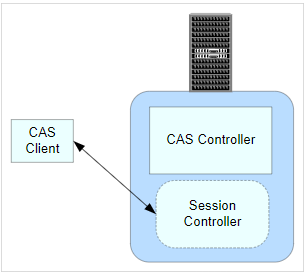
\includegraphics[scale = 0.8]{images/smp_server.png}
    \caption{Single-machine CAS Server \textcolor{red}{(STOLEN EXAMPLE)} }
    \label{SMP Achitecture}
\end{figure}

\subsubsection{Massively Parallel Processing (MPP)}
Massively Parallel Processing (MPP) is an environment where a distributed CAS server consists of one controller, one or more workers, and one backup controller (optional), each running on a separate machine. In a distributed server (MPP mode), a session process is created on each machine in the cluster. These processes are sometimes referred to as the session controller and session worker processes. Even though the sessions have their own operating system processes, the server processes must continue to run. When the server process terminates, the session processes also terminate.

\begin{figure}[H]
    \centering
    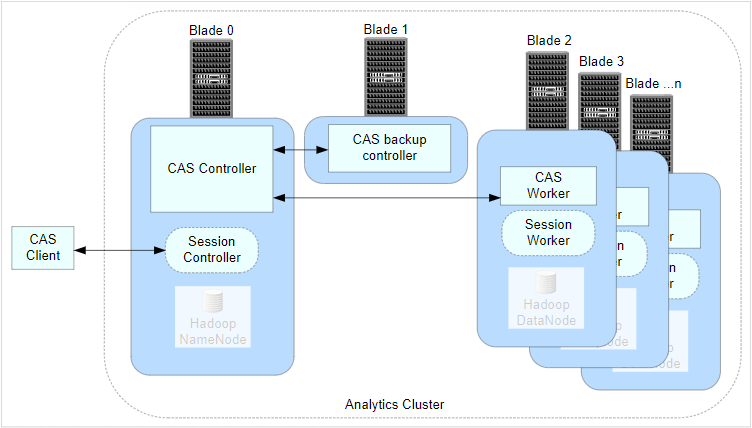
\includegraphics[scale = 0.8]{images/mpp_server.png}
    \caption{Distributed CAS Server \textcolor{red}{(STOLEN EXAMPLE)} }
    \label{MMP Architecture}
\end{figure}

